\chapter{Result}
This chapter presents the results from the conducted evaluation. Appendix \ref{appendix:raw} contains raw data and metrics over data that may not been presented in this chapter.

\todo[inline]{Todo: Write summary of what to come in chapter. }

\section{Performance Overhead}
The results from benchmarking the application on DaCapo Benchmark Suit \parencite{dacapo} is seen in Figure \ref{fig:Time} and \ref{fig:Memory}. Both graphs are constructed to show the added overhead of running the applications with Dynamic Taint Tracking activated. The graphs are conducted based on the data in Table \ref{TimeTable} and \ref{MemoryTable}.


\subsection{Time}
Figure \ref{fig:Time} displays the results of the average time overhead per application. The results show that the application with the least average time overhead was Tradesoap where 14.7\% was added. The largest application however, was Fop with an additional of 426.2\%. The average overall overhead is 142.1\%.

From the Tables \ref{TimeTable} can we as well see that the variation between the minimum and maximum time will for all applications be 437.8\%.

\begin{figure}[H]
	\centering
	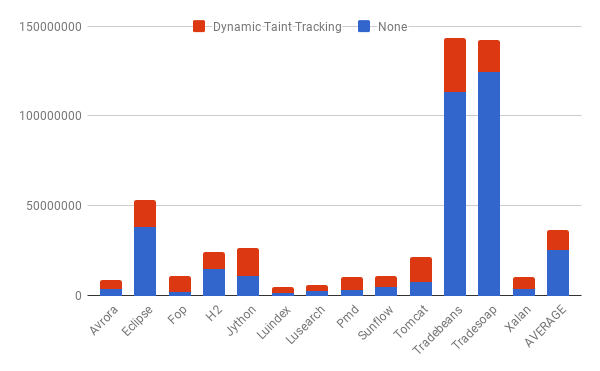
\includegraphics[width=\textwidth]{images/Time.png}
	\caption{Average Added Time in Microseconds}
	\label{fig:Time}
\end{figure}


\subsection{Memory}
Figure \ref{fig:Memory} displays the results of the average memory overhead per application. The results show that the application with the least average memory overhead was Eclipse where 5.5\% was added. The largest application however, was Fop with an additional of 277.8\%. The average overall overhead is 127.2\%.

From the Table \ref{MemoryTable} can we as well see that the variation between the minimum and maximum memory will for all 305.3\%.

\begin{figure}[H]
	\centering
	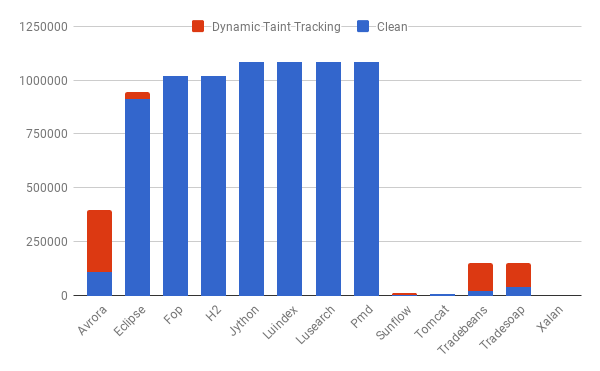
\includegraphics[width=\textwidth]{images/Memory.png}
	\caption{Average Added Memory in Kilobytes}
	\label{fig:Memory}
\end{figure}



\section{Applications}
Table \ref{table:MicroTable} shows the vulnerabilities from running Stanford SecuriBench Micro \parencite{securiBenchMicro} with and without Dynamic Taint Tracker. In the table can we see that an prevention rate of 100\% is reached with Dynamic Taint Tracker activated.

\begin{table}[H]
  \centering
  \caption{Security Vulnerabilities Found in Stanford SecuriBench Micro}
  \label{table:MicroTable}
    \begin{tabular}{rcc}
      & \textbf{None} & \textbf{Dynamic Taint Tracking} \\
      \textbf{Cross Site Scripting (Reflected)} & 71            & 0  \\
      \textbf{SQL Injection}                    & 20            & 0  \\
      \textbf{Buffer Overflow}                  & 1             & 0  
    \end{tabular}
\end{table}


Table \ref{table:InsecureTable} shows the vulnerabilities from running Insecure \parencite{insecure} with and without Dynamic Taint Tracker. The prevention rate of using Dynamic Taint Tracker is overall 75\%. 

\begin{table}[H]
  \centering
  \caption{Security Vulnerabilities Found in Insecure}
  \label{table:InsecureTable}
    \begin{tabular}{rcc}
      & \textbf{None} & \textbf{Dynamic Taint Tracking} \\
      \textbf{Cross Site Scripting (Reflected)}      & 2             & 2  \\
      \textbf{SQL Injection - Authentication Bypass} & 2             & 0  \\
      \textbf{SQL Injection - Hypersonic SQL}        & 4             & 0  
    \end{tabular}
\end{table}


The results from evaluating the application SnipSnap \parencite{snipsnap} is seen in Table \ref{table:SnipSnapTable}. Here is the overall prevention rate 77.2\%.

\begin{table}[H]
  \centering
  \caption{Security Vulnerabilities Found in SnipSnap}
  \label{table:SnipSnapTable}
  \begin{tabular}{rcc}
    & \textbf{None} & \textbf{Dynamic Taint Tracking} \\
    \textbf{Cross Site Scripting (Reflected)}      & 172           & 39   \\
    \textbf{CRLF Injection}                        & 3             & 0    \\
    \textbf{SQL Injection}                         & 47            & 10   \\
    \textbf{SQL Injection - Authentication Bypass} & 2             & 2       
  \end{tabular}
\end{table}


Table \ref{table:Ticketbook} shows the vulnerabilities from evaluating Ticketbook \parencite{ticketbook} with and without Dynamic Taint Tracking. The overall prevention rate is 73.3\%.

\begin{table}[H]
  \centering
  \caption{Security Vulnerabilities Found in Ticketbook}
  \label{table:Ticketbook}
  \begin{tabular}{ccc}
    & \textbf{None} & \textbf{Dynamic Taint Tracking} \\
    \textbf{Cross Site Scripting (Persistent)} & 2             & 0 \\
    \textbf{Cross Site Scripting (Reflected)}  & 12            & 4 \\
    \textbf{SQL Injection}                     & 1             & 0
  \end{tabular}
\end{table}